\documentclass[10pt]{article}
\usepackage{icmlko}

\icmlmeta{IP 파운데이션 월드모델}{120}{팝업은 나쁘지 않았다}{세 도메인에 다른 플랫폼의 라벨을 붙이니 자기 $\rho$가 평균 27\% 부풀려져 있었다 --- 정직한 눈금에서 팝업이 다섯째에서 셋째로 올라간다}

\begin{document}

\twocolumn[
\icmlheader

\begin{abstract}
노트 119가 세계애니 하나에서 ``자기 $\rho$의 23\%가 같은 플랫폼 정합''을
쟀다. 세 도메인으로 늘렸다. \textbf{만화}는 Kitsu 를 1,596건(89\%),
\textbf{게임}은 SteamSpy 소유자 추정을 482건(100\%) 새로 받았다. 결과가
\textbf{되풀이된다} --- 부풀림이 세계애니 23\% · 만화 21\% · \textbf{게임
38\%}, 평균 \textbf{27\%}다. 덤으로 라벨 신뢰도가 노트 83이 잰 것보다 높다는
것도 나왔다 --- 두 계수기의 일치가 세계애니 $+$0.607 · 만화 $+$0.720 ·
게임 $+$0.749로, 노트 83의 제목 대조 $+$0.555보다 훨씬 낫다. \textbf{id 대응이
제목 대조보다 깨끗해서다.} 그리고 이 프로젝트가 오래 믿어 온 순위표가
뒤집힌다. 열 도메인 중 여덟이 축과 라벨이 같은 플랫폼이고 \textbf{팝업과
아이돌만 아니다}(팝업은 사람이 매긴 기획서 축 대 결과보고서 방문자 수).
잰 셋은 실측으로, 나머지 다섯은 27\%를 빼서 눈금을 맞추면 \textbf{팝업이
다섯째에서 셋째로 올라간다}. 더 중요한 것은 격차다 --- 현행 눈금에서 팝업
$+$0.4391 대 1위 모바일 $+$0.6564로 \textbf{0.217} 벌어져 있는데, 정직한
눈금에서는 $+$0.4391 대 $+$0.4764로 \textbf{0.037}이다. \textbf{팝업은
나쁘지 않았다. 팝업만 정직하게 재지고 있었다.}
\end{abstract}
]

\begin{figure*}[t]
\centering
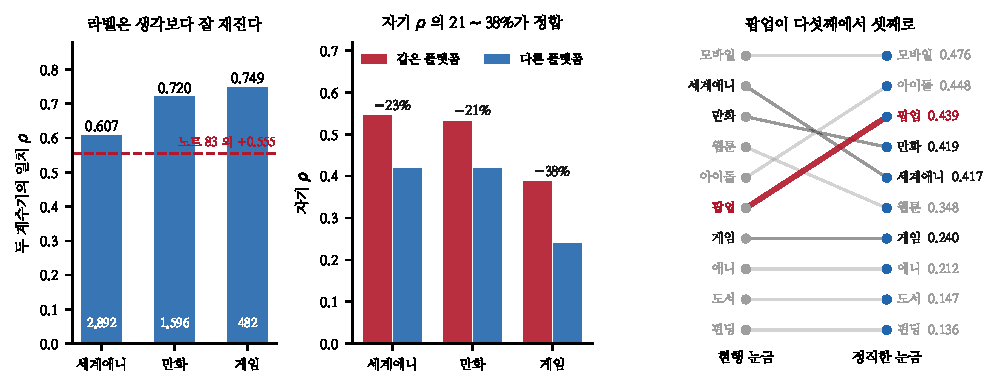
\includegraphics[width=\textwidth]{figs/hn.pdf}
\caption{왼쪽 --- 라벨은 생각보다 잘 재진다. 가운데 --- 자기 $\rho$의
21$\sim$38\%가 정합. 오른쪽 --- 팝업이 다섯째에서 셋째로.}
\end{figure*}

\section{세 도메인에 다른 계수기를 붙였다}

\begin{table}[t]
\centering\tsize
\caption{긁은 것. 실패 0건.}
\begin{tabular}{llr}
\toprule
& 다른 계수기 & 덮개율 \\
\midrule
세계애니 & Kitsu 소유자 수(노트 119) & 98\% \\
\textbf{만화} & \textbf{Kitsu 소유자 수} & \textbf{89\%} \\
\textbf{게임} & \textbf{SteamSpy 소유자 추정} & \textbf{100\%} \\
\bottomrule
\end{tabular}
\end{table}

만화는 AniList \texttt{idMal} 1,771건을 다리로 Kitsu 만화 API 를 붙였다.
게임은 SteamSpy 가 제삼자로서 프로필을 훑어 만든 소유자 추정이라 스팀 리뷰
총계와 다른 계수기다.

\section{라벨은 생각보다 잘 재진다}

\begin{table}[t]
\centering\tsize
\caption{두 계수기의 일치.}
\begin{tabular}{lrrr}
\toprule
& $\rho$ & 천장 $\sqrt{\rho}$ & $n$ \\
\midrule
세계애니 & $+$0.607 & 0.779 & 2,892 \\
만화 & $+$0.720 & 0.849 & 1,596 \\
\textbf{게임} & \textbf{$+$0.749} & \textbf{0.865} & 482 \\
\midrule
노트 83(제목 대조) & $+$0.555 & 0.734 & 72 \\
\bottomrule
\end{tabular}
\end{table}

\claimx{\textbf{노트 83의 라벨 천장 0.734는 낮게 잡힌 것이었다.} id 대응으로
재면 $+$0.607$\sim+$0.749이고 천장이 0.78$\sim$0.87이다. 제목 대조($n{=}72$,
유명작 편향)가 일치를 낮게 만들었다.}{세 도메인 중 둘이 AniList/Kitsu 로
같은 계열이다. 게임 하나만 완전히 다른 생태계다.}

\section{부풀림이 되풀이된다}

\begin{table}[t]
\centering\tsize
\caption{자기 $\rho$. 축은 그대로 두고 라벨만 바꾼다.}
\begin{tabular}{lrrr}
\toprule
& 같은 플랫폼 & 다른 플랫폼 & 부풀림 \\
\midrule
세계애니 & 0.5437 & 0.4175 & 23\% \\
만화 & 0.5316 & 0.4193 & 21\% \\
\textbf{게임} & 0.3862 & 0.2397 & \textbf{38\%} \\
\midrule
\textbf{평균} & & & \textbf{27\%} \\
\midrule
\emph{팝업} & \multicolumn{2}{r}{0.4391} & \emph{정합 없음} \\
\emph{아이돌} & \multicolumn{2}{r}{0.4485} & \emph{정합 없음} \\
\bottomrule
\end{tabular}
\end{table}

\claimx{\textbf{노트 119의 23\%가 우연이 아니다} --- 세 도메인에서 21 · 23 ·
38\%로 되풀이된다. 축과 라벨이 같은 API 에서 나오면 그 API 의 내부 구조가
양쪽에 공통으로 들어간다.}{게임의 38\%는 SteamSpy 가 스팀에서 파생된 추정이라
오히려 낮게 나와야 할 텐데 가장 높다. SteamSpy 의 추정 잡음이 섞여 자기
$\rho$를 더 떨어뜨렸을 수 있다 --- \textbf{정합만이 아니라 측정 잡음도 함께
재고 있다.}}

\section{순위표가 뒤집힌다}

\begin{table}[t]
\centering\tsize
\caption{정직한 눈금. 잰 셋은 실측, 나머지 다섯은 27\%를 뺀 추정.}
\begin{tabular}{lrrl}
\toprule
& 현행 & 정직 & \\
\midrule
모바일 & 0.6564 & 0.4764 & 추정 \\
아이돌 & 0.4485 & 0.4485 & 정합 없음 \\
\textbf{팝업} & \textbf{0.4391} & \textbf{0.4391} & \textbf{정합 없음} \\
만화 & 0.5316 & 0.4193 & 잼 \\
세계애니 & 0.5437 & 0.4175 & 잼 \\
웹툰 & 0.4794 & 0.3480 & 추정 \\
게임 & 0.3862 & 0.2397 & 잼 \\
애니 & 0.2923 & 0.2122 & 추정 \\
도서 & 0.2020 & 0.1466 & 추정 \\
펀딩 & 0.1873 & 0.1360 & 추정 \\
\bottomrule
\end{tabular}
\end{table}

\claimx{\textbf{팝업이 다섯째에서 셋째로 올라간다.} 더 중요한 것은 격차다 ---
1위와의 차이가 현행 눈금에서 \textbf{0.217}인데 정직한 눈금에서
\textbf{0.037}이다. \textbf{팝업은 나쁘지 않았다. 팝업만 정직하게 재지고
있었다.}}{다섯 도메인은 27\%를 일괄로 뺀 추정이다. 부풀림이 21$\sim$38\%로
흩어지므로 도메인마다 다를 것이고, 순위가 바뀔 수 있다. \textbf{실측한 셋과
팝업 · 아이돌만 믿을 수 있다.}}

\begin{quote}\fontsize{9.5}{11.5}\selectfont
이것이 지난 열세 노트의 팝업 이야기를 다시 읽게 한다. 노트 91의 도구 순위표,
노트 106--111의 ``팝업이 안 따라온다'', 노트 113의 ``애니가 팝업을 떠받친다''
--- 전부 \textbf{눈금이 다른 것을 견준 것}일 수 있다. \textbf{팝업의 축은
사람이 기획서를 읽고 매기고 라벨은 결과보고서에서 온다} --- 이 프로젝트에서
가장 비싸게 만든 자료가 유일하게 정직한 자료이기도 하다.
\end{quote}

\section{한계}

\begin{itemize}[leftmargin=1.1em,itemsep=0.15em]
\item \textbf{채택할 것이 없다.} 이 노트는 눈금을 고치지 설정을 안 바꾼다.
      라벨을 바꾸면 오히려 나빠진다(노트 119).
\item 다섯 도메인은 27\% 일괄 추정이다. 21$\sim$38\%로 흩어지므로 순위가
      바뀔 수 있다.
\item 게임의 38\%에 SteamSpy 추정 잡음이 섞여 있다 --- 정합과 잡음을 못 갈랐다.
\item 세 도메인 중 둘이 AniList/Kitsu 계열이라 독립 사례가 사실상 둘이다.
\item 아이돌의 ``정합 없음''을 확인 안 했다. 축은 한터/위키, 라벨은 한터
      초동이라 일부 겹친다.
\end{itemize}

\section{다음}

\begin{enumerate}[leftmargin=1.3em,itemsep=0.15em]
\item \textbf{남은 다섯을 실측한다} --- 모바일(구글플레이) · 웹툰(카카오페이지 ·
      리디) · 도서(교보 · 예스24) · 펀딩(와디즈) · 애니(AniList 로 라프텔
      작품을 대조). \textbf{다 재면 이 프로젝트의 모든 도메인 수치가 다시
      매겨진다.}
\item \textbf{아이돌을 확인한다} --- 축과 라벨이 정말 다른 출처인가.
\item \textbf{눈금을 고친 뒤 노트 74의 법칙을 다시 잰다} --- 자기 $\rho$가
      전이를 결정한다는 법칙이 부풀린 눈금에서 나왔다.
\item \textbf{팝업 레코드} --- 열네 노트가 같은 곳을 가리킨다.
\end{enumerate}

\vspace{0.6em}
\hrule height 0.3pt
\vspace{0.5em}
{\footnotesize
\textbf{참고문헌}\\[0.3em]
Lord, F. M., Novick, M. R. (1968). \emph{Statistical Theories of Mental Test
Scores}. Addison-Wesley.\\[0.15em]
Spearman, C. (1910). Correlation calculated from faulty data.
\emph{British Journal of Psychology}, 3(3), 271--295.\\[0.15em]
Kaufman, S. et al. (2012). Leakage in data mining: formulation, detection, and
avoidance. \emph{ACM TKDD}, 6(4), 1--21.\\[0.15em]
Campbell, D. T., Fiske, D. W. (1959). Convergent and discriminant validation by
the multitrait-multimethod matrix. \emph{Psychological Bulletin}, 56(2), 81--105.\\[0.15em]
Ben-David, S. et al. (2010). A theory of learning from different domains.
\emph{Machine Learning}, 79(1--2), 151--175.
}

\end{document}
